\documentclass[11pt]{article}

\usepackage{microtype}
\usepackage{amsmath}
\usepackage{float}
\usepackage[colorlinks, urlcolor = blue]{hyperref}

\usepackage{graphicx}
\usepackage{caption}
\usepackage{subcaption}

\title{\textbf{Motion Estimation from optical flow}}
\author{ Moritz Loos 112385 }
\date{ Winter term 2014/15 }
\begin{document}
	
	\maketitle

	\section{Abstract}
	The goal of the project was to estimate the motion of a uav that is equipped with a stereo camera system with help of the optical flow in the stereo images.

	\section{Introduction}
	optical flow is the tracking of points from frame to frame. there are two possible approaches:
	First try to track every single pixel or in a defined interval from frame to frame. Second try to track features from frame to frame (feature-based matching).
	
	\begin{figure}[ht!]
		\centering
		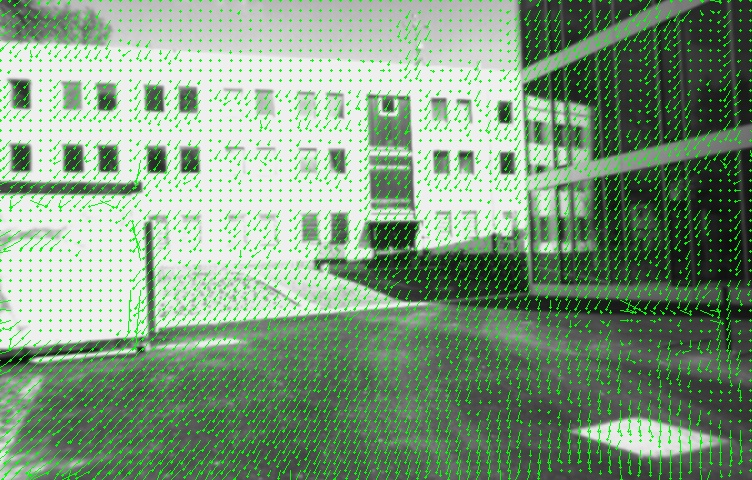
\includegraphics[width=90mm]{images/farneback.jpg}
		\caption{Optical flow field \label{overflow}}
	\end{figure}
	
	\begin{figure}[ht!]
		\centering
		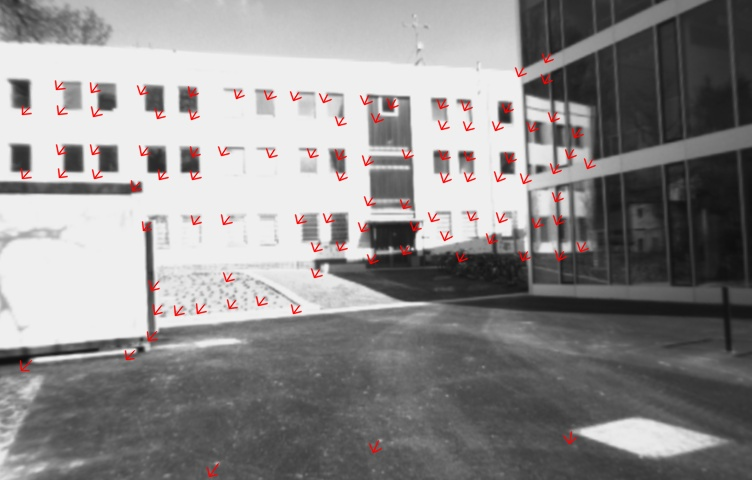
\includegraphics[width=90mm]{images/feature-based-matching.jpg}
		\caption{Optical flow field \label{overflow}}
	\end{figure}
	
	Probably they have some advantages and disadvantages. Obviously you have with the optical field approach much more points and especially a better distribution of points, but it is much more slower and has much more outliers. i decided to use the feature-based matching because it is much more stable and faster than the other approach.
	unfortunately a simple mapping of optical flow vectors to the motion of the camera is only possible under specially constraints that we can’t hold: The scene have to be static and have to lie parallel to the image plane of the camera and in a defined height. That means the camera have to look permanent down.
	
	\begin{figure}[ht!]
		\centering
		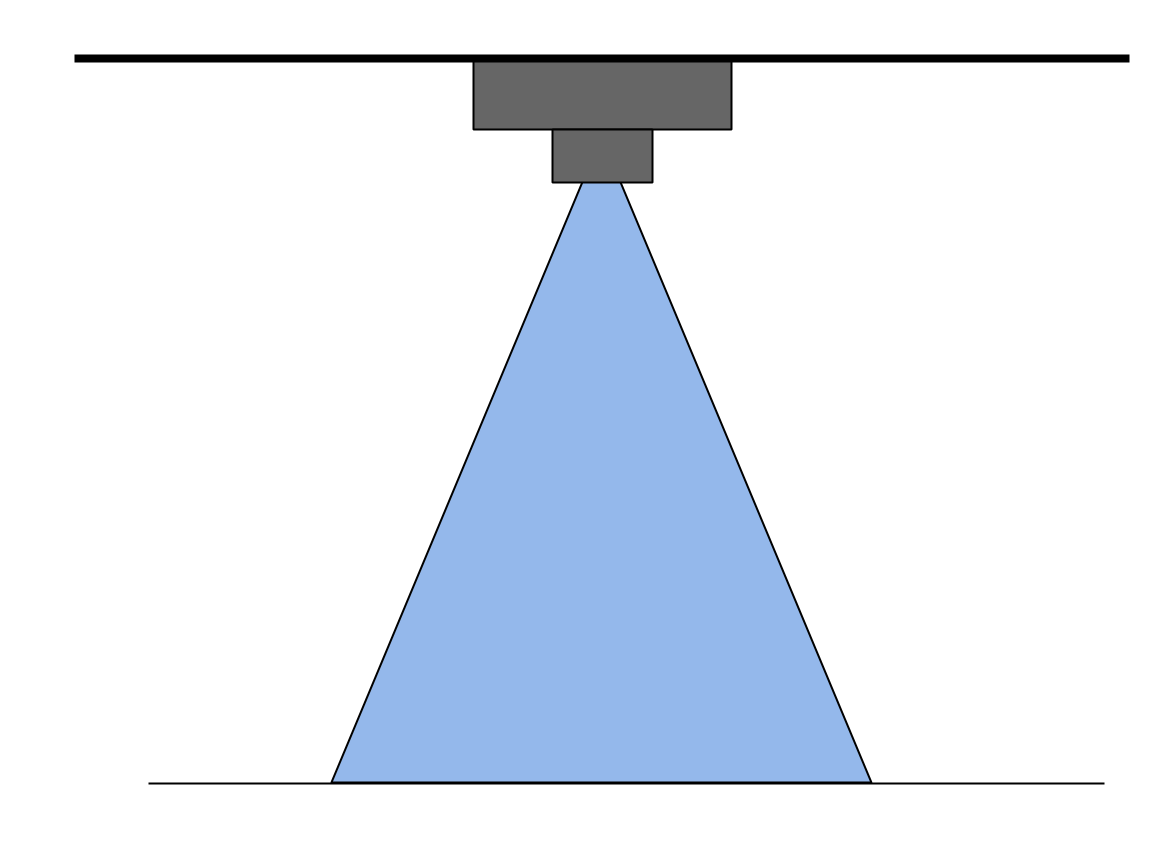
\includegraphics[width=90mm]{images/look_down.png}
		\caption{constraint: camera parallel to the ground plane \label{overflow}}
	\end{figure}
	
	If this constraints are given you could estimate the motion using the length and direction of the optical flow vectors. [http://cvpr.uni-muenster.de/teaching/ss09/computerVisionSS09/script/CV08-Bewegungsanalyse.pdf]
	
	\begin{figure}[ht!]
		\centering
		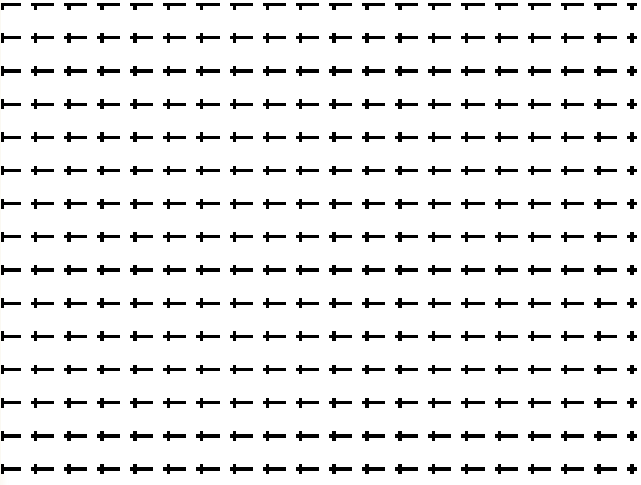
\includegraphics[width=90mm]{images/translation.png}
		\caption{translation \label{overflow}}
	\end{figure}
	
	\begin{figure}[ht!]
		\centering
		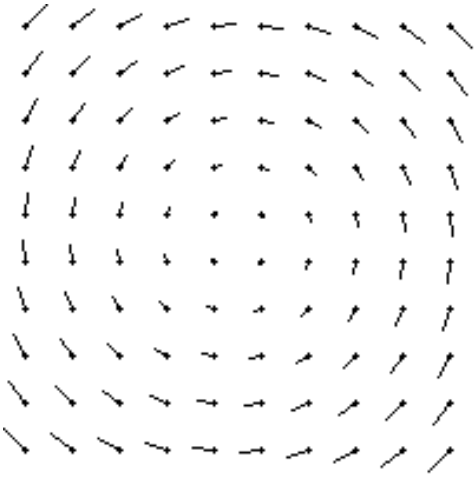
\includegraphics[width=90mm]{images/rotation.png}
		\caption{rotation \label{overflow}}
	\end{figure}
	
	
	Because we can’t hold this constraints we had to find other approaches.
	
	\section{Settings}
	our system is a calibrated stereo rig [hagen paper] and all values are defined like follows:
	
	\begin{figure}[ht!]
		\centering
		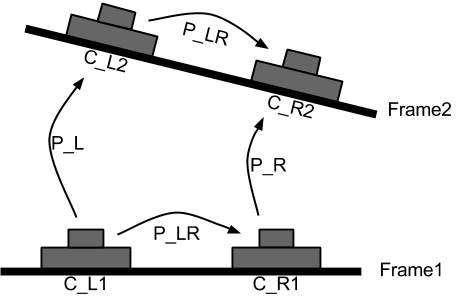
\includegraphics[width=90mm]{images/camera setup.png}
		\caption{rotation \label{overflow}}
	\end{figure}

	P represent the projection matrix of the current camera (P\_L is the projection matrix from the left camera in frame 1 to the left camera in frame 2). C represent the current camera image.

	I am using the opencv library.
	
	\section{Visual odometry}
	to estimate the motion we need to find corresponding points in all 4 images. My approach for performing visual odometry is represented in figure [] and is explained in the following.
	
	\begin{figure}[ht!]
		\centering
		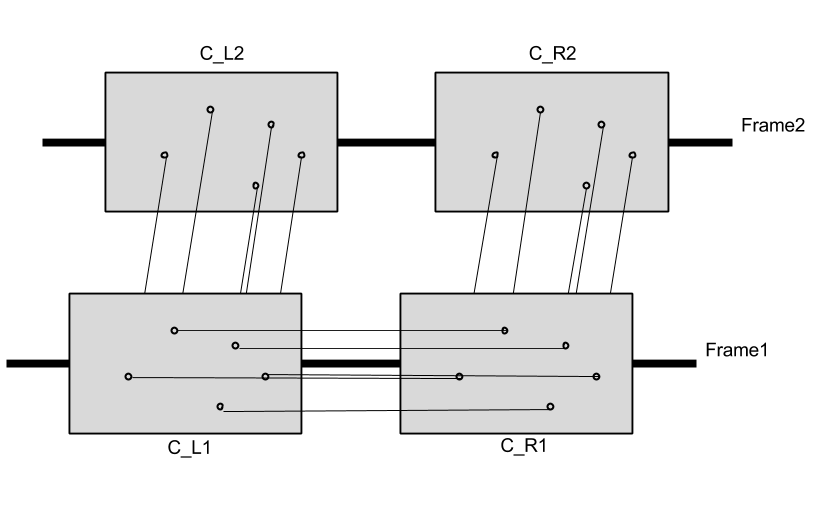
\includegraphics[width=90mm]{images/setup.png}
		\caption{rotation \label{overflow}}
	\end{figure}
	
	I start to detect features in C\_L1 with the Shi-Tomasi Corner detector that is implemented in OpenCV. The Shi-Tomasi approach is a faster and more stable modification from Harris Corner detector. It is using the eigenvalues to decide if the point is a corner, an edge or neither of them. The Shi-Tomasi Corner detector is a really common approach, but an alternate could be the FAST feature detector or SURF (Speeded-Up Robust Features).
	[http://www.aishack.in/tutorials/the-shitomasi-corner-detector/, http://www.cs.ucf.edu/~mtappen/cap5415/lecs/lec5.pdf, http://www.informatikprojekt.de/uploads/dbv\_report.pdf]
	After I found the features in C\_L1 I try to find them in C\_R1 and C\_L2. The correspondence points that i found in C\_R1 I try to find them in C\_R2. 
	My approach to refind points is using the lucas kanade algorithm that is implemented in openCV as well. 
	[http://www.informatikprojekt.de/uploads/dbv\_report.pdf]
	The Lucas Kanade is beside SURF one of the most common algorithm to find features in an image. This method expects that the intensity of a point and the points in a specified window range don’t change from frame to frame. That's why this algorithm works well only for small motion (high fps). 
	
	In this project we used the pyramidical approach of this algorithm. Therefore the reference images is downscaled to a certain number of pyramidal layers showed in figure []. Than the lucas kanade tracking algorithm is called on each layer with a different resolution in ascending direction and only in the previously found range. With this approach the algorithm is faster, more robust and provide better accuracy. [http://tu-dresden.de/die\_tu\_dresden/fakultaeten/fakultaet\_forst\_geo\_und\_hydrowissenschaften/fachrichtung\_geowissenschaften/ipf/photogrammetrie/dateien/Westfeld2004.pdf]
	
	\begin{figure}[ht!]
		\centering
		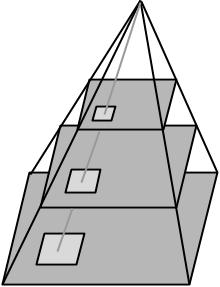
\includegraphics[width=90mm]{images/pyramidical.png}
		\caption{pyramedical approach of lucas kanade \label{overflow}}
	\end{figure}
	
	To prevent wrong connections of point we have to delete outlier. therefore opencv gives us the chance to find inliers with RANSAC in the findfundamentalMat() method. But this inlier estimation didn’t works as good as expect. Too many good points are defined as outliers and some bad points retains as inliers. And because it is so difficult to retrace why they are defined like this that we hat to define inliers by our own. A really good approach is to use the constraint of our rectified stereo camera system. The flow vectors from C\_L1 to C\_R1 and from C\_L2 to C\_R2 have to lie horizontally on the images. Is this not the case we delete this point in all four frames. Sometimes there are still some wrong classifications but it fits for us.
	In following figure the green arrows shows the inliers and die red ones the outliers.
	
	\begin{figure}[ht!]
		\centering
		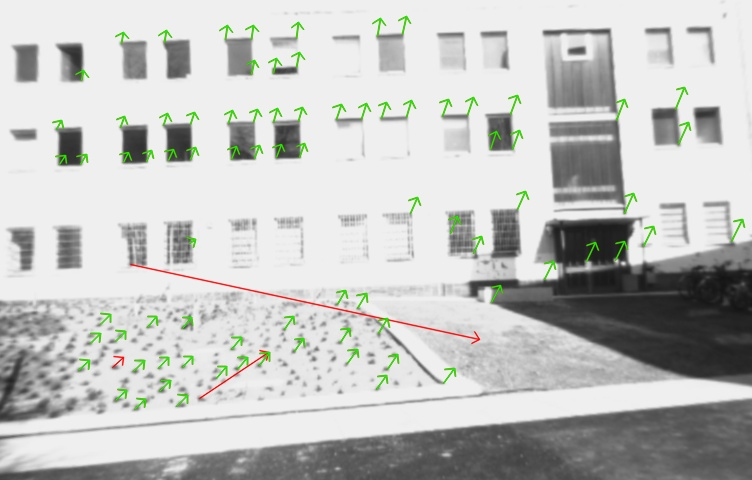
\includegraphics[width=90mm]{images/inlier_outlier3.jpg}
		\caption{inlier (green) and outlier (red) \label{overflow}}
	\end{figure}
	
	\section{Motion Estimation}
	
	There are many different approaches to estimate the motion. 
	When we have again a look to our camera setup (figure []) it becomes clear that we have to compute the projection matrices P\_L and P\_R. These matrices can be computed from the essential matrix. The first step is to compute the fundamental matrix for the left and the right camera each from frame 1 to frame 2. Therefore we need correspondence points in all four frames and use the opencv implementation findfundamentalmat(). The second step is to compute the essential matrix using the fundamental and the calibration matrix. The formula is E = K’ * F * K [from hartley and zisserman].
	To obtain the perspective matrix we have to decompose the essential mat using svd [referenz auf irgendein paper].
	unfortunately the essential mat can be decomposed to 4 different projection matrices and we have to find the right on. Therefore the points are triangulated with all four possible projection matrices and if all points are in front of both cameras you found the right one. 
	
	\begin{figure}[ht!]
		\centering
		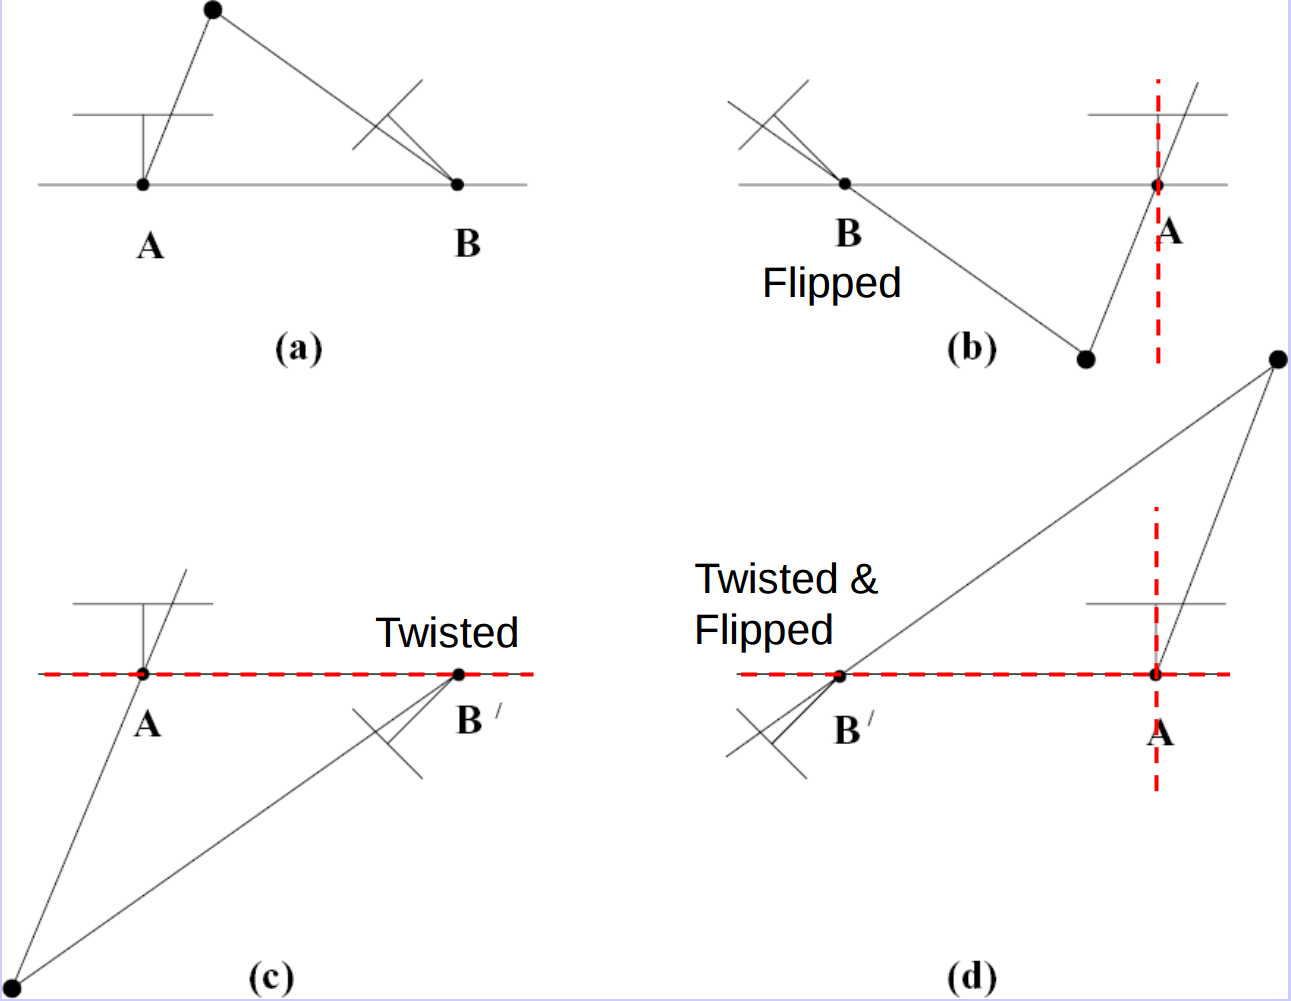
\includegraphics[width=90mm]{images/possible_P_Mats.png}
		\caption{inlier (green) and outlier (red) [© Volker Rodehorst - Lecture Photogrammetric Computer Vision - WS 14/15]
			 \label{overflow}}
	\end{figure}
	One problem left is that the found projection matrix is up to scale. that means we get only the normalized direction vector of both cameras.
	The approach to compute the right scale factors for both cameras is to triangulate a reference point cloud from the left to the right camera called X. This point cloud is already right scaled because it is computed from P\_LR that is given from the stereo calibration and is already in metrical form. Than we triangulate points from first left to second left camera (X\_L) and from first right to second right camera (X\_R).  To estimate the scale factor for left and right camera we can just compare each point cloud with the reference point cloud X like following:
	[gleichung 1], [gleichung 2].  [Paper Rodehorst].
	
	there exist many approaches to estimate the motion of a stereo camera based system beside the essential mat method we had an look to two other ones.
	
	First It is possible to estimate the motion with the Perspective-n-point approach. Therefore you have to find 3D point to 2d image point correspondences. Easy to receive from triangulation. This approach is also implemented in OpenCV. Fortunately also as a Ransac implementation. [http://homepages.inf.ed.ac.uk/rbf/CVonline/LOCAL\_COPIES/MARBLE/high/pia/solving.htm]
	
	Second approach is to compare the orientation of the pointcloud triangulated in frame 1 to the point cloud triangulated in frame 2. This method is explained in following paper [Combining Stereo Vision and Inertial Navigation System]
	
	\section{Results}
	we get some useful results for the first two approaches, but with a to high error consumption. Our accuracy after 100 meters is +-10 meters in all directions.
	To compare all 3 methods our implementation is not robust enough and have to be improved.
	
	
	\section{Future work}
	To robust the algorithm it is necessary to minimize the error from frame to frame. A probably useful approach could be a bundle adjustment. After that a comparison of all 3 methods could be useful to decide which one to use or to compare two / three of them to get more stable results.
	furthermore until now the implementation is based on usability and comfort. To run this code on the uav it should be improved concerning the performance especially it should testet live.
	
		
	
	
\end{document}